\documentclass[12pt]{article}
\usepackage{graphicx}
\usepackage{amsmath}

\usepackage[margin=1in]{geometry}
\usepackage{float}
\usepackage{listings}
\usepackage{booktabs}

\title{Labwork 6: Map}
\author{Ngo Quang Truong 2540106}
\date{3 Oct 2026}

\begin{document}

\maketitle
\newpage

\section{Introduction}
This report presents three image-processing operations implemented: grayscale binarization, brightness control, and blending two images on GPU.

\section{Method}
For an array $A$ and a function $f$, the Map pattern is defined as
\begin{equation}
map(A,f) = [f(x_i), \; \forall x_i \in A]
\end{equation}
A $16\times16$ thread block is used for all three labworks. Test image: a $3840\times2160$ RGB image.

\section{Grayscale Binarization}
Each pixel's RGB value is first averaged into a grayscale intensity $\Phi(x,y)$, then thresholded against $\tau = 128$:
\begin{equation}
b(x,y) = \begin{cases} 0 & \Phi(x,y) < \tau \\ 255 & \Phi(x,y) \geq \tau \end{cases}
\end{equation}

\begin{figure}[H]
    \centering
    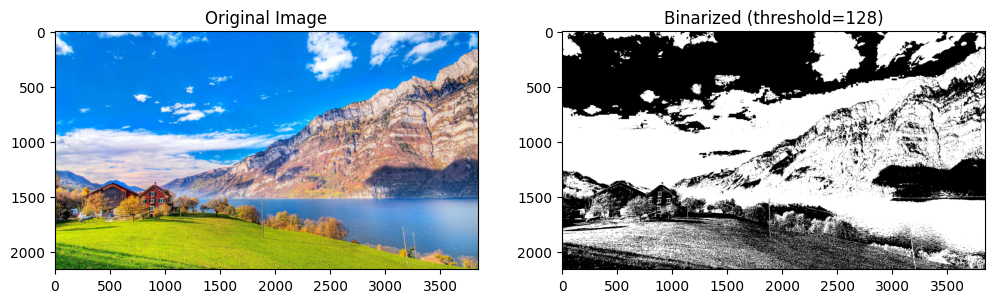
\includegraphics[width=\textwidth]{binarization_output.png}
    \caption{Original image vs.\ binarized output}
    \label{fig:binarization}
\end{figure}

\section{Brightness Control}
Each channel of each pixel is shifted by a constant and clamped back into the valid $[0,255]$ range:
\begin{equation}
I'(x,y) = \min(\max(I(x,y) + \beta,\ 0),\ 255)
\end{equation}
with $\beta = 50$.

\begin{figure}[H]
    \centering
    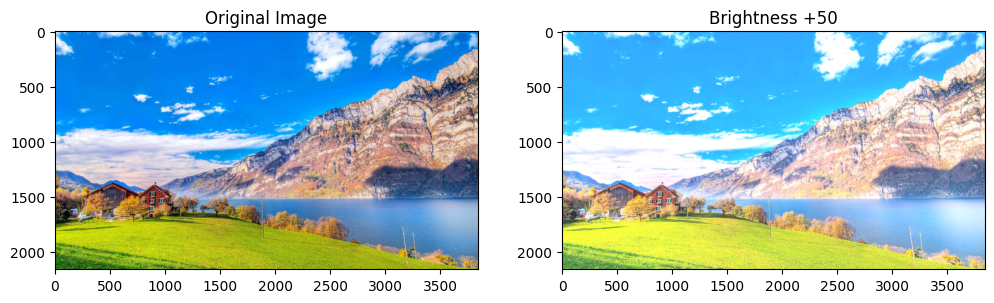
\includegraphics[width=\textwidth]{brightness_output.png}
    \caption{Original image (left) vs.\ brightness adjusted output}
    \label{fig:brightness}
\end{figure}

\section{Blending Two Images}
Two same-size images $\Phi_1$ and $\Phi_2$ are combined per-channel using a weight $c$:
\begin{equation}
Q(x,y) = c \times \Phi_1(x,y) + (1-c) \times \Phi_2(x,y)
\end{equation}
The second image was generated by horizontally flipping the original ($c = 0.5$).

\begin{figure}[H]
    \centering
    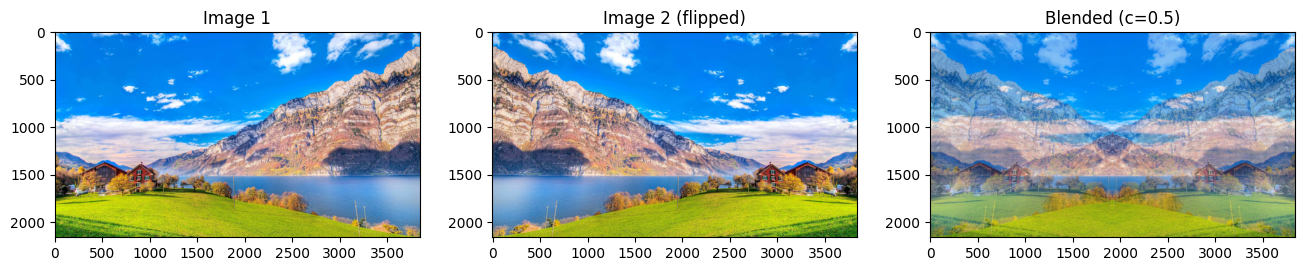
\includegraphics[width=\textwidth]{blending_output.png}
    \caption{Image 1 (left), Image 2 / flipped}
    \label{fig:blending}
\end{figure}

\section{Results}

\begin{table}[H]
\centering
\begin{tabular}{lc}
\toprule
Labwork & GPU time (s) \\
\midrule
6a: Binarization & 2.1619 \\
6b: Brightness control & 0.1451 \\
6c: Blending & 0.2114 \\
\bottomrule
\end{tabular}
\caption{Execution time.}
\label{tab:results}
\end{table}


\end{document}
